

% The DBpedia knowledge base has several advantages over existing knowledge bases: it covers many domains; it represents real community agreement; it automatically evolves as Wikipedia changes, and it is truly multilingual. The DBpedia knowledge base allows you to ask quite surprising queries against Wikipedia

% % The DBpedia ontology provides the classes and properties used in the DBpedia knowledge graph. DBpedia ontology can be differentiated into the raw extraction of Wikipedia dumps and the mapping based extraction which is based on the mappings between info-boxes and their ontology. \textbf{http://dbpedia.org/property/, (prefix dbp)} represents properties extracted from the raw info-box extraction and \textbf{http://dbpedia.org/ontology/, (prefix dbo)} represents the DBpedia ontology. \textbf{http://dbpedia.org/resource/, (prefix dbr)} represents the DBpedia resource.
TagMe is a popular Entity Linking tool explicitly released for short texts\cite{tagme}.Falcon performs joint entity and relation linking of a short text by leveraging principles like compounding, headword identification


We use these sentences within several statistical and embedding approaches to map relations in the knowledge graph to the tokens in the natural language question.
 
 
 
 
 In future work, we attempt to construct a domain knowledge graph from the specific business, and reduce the noise in the general knowledge graph, which may have better results and have certain practical significance. The model also will be fine-tuned in order to achieve more compelling results so a more comprehensive quantitative comparison will be performed.
 
 
 
 
% This list is merged top k $P_{Final}$ relations for each keyword in the question. This Candidate list is $Candidate\_List_{First\cap}$ for the First hop relations and the Final Intersection, $Candidate\_List_{Final\cap}$.
 
 A particular innovation of our approach in this context is that we use both character- and word-level in- formation from the question for both entity and predicate prediction. Character-level modelling of questions (or en- tity mentions) and entities has been shown advantageous for this task because of its out-of-vocabulary (OOV) word handling abilities [12, 26]. However, the downside of purely character-level models is their inability to exploit word-level semantics (as captured in word embeddings [17]), which are useful for modelling questions, predicates and types. Our model combines the OOV-related advantages of character- level models and the rich semantics of word-level models. In this respect, our work is close to that of Yin et al. [26], with the difference that our approach employs a single question representation network and is less specific for simple ques- tions since it does not split the question into mention-pattern pairs.
 
 
 explain simple and complex questions in intro
 
 Additionally, our approach can be used to answer compositional questions despite never having seen such questions at training time.
 
 In this paper, we focus on the challenges of natural language processing over knowledge graphs of scientific datasets. In particu- lar, we introduce Bio-SODA, a natural language processing engine that does not require training data in the form of question-answer pairs for generating SPARQL queries. Bio-SODA uses a generic graph-based approach for translating user questions to a ranked list of SPARQL candidate queries.
 
 
 Some of the challenges faced by QA systems are:
• Lexical gap – surface forms for relations expressed in a question can be quite different from those used in the KG,
• Ambiguity – the same word is used for different entities, such as president of a company or a country,
• Unknown knowledge boundaries – QA systems can of- ten hardly decide whether a certain question is answer- able at all give a certain knowledge base. 
% used by Neural Network-based Question Answering over Knowledge Graphs on Word and Character Level

Prior to the availability of query logs, query expansion methods suggested terms and phrases using, for example, relevance feedback [26], concept hierarchies [44] and over-representation statistics [9]. More recently, query expansion methods have used word embed- dings [37] to suggest search terms that are semantically similar to the search query. For this purpose, embedding models have been trained on the entire corpus [27], search results [12] and on the basis of document relevance, rather than term proximity [50]. 


In this age of online retrieval, it's only reasonable to provide assistance to consumers who want to enhance their queries. Short lists of suggested terms obtained from comments, nearest neighbours, and term variants of original query terms could be one form of such guidance.


A major problem with the interactive approach to IR is being able to gain an understanding of the nature of the tion itself, and then to move from such under- standing to the specification of a system design and structure that supports and enhances it.

used a graph composed by sentences, linked to both the belonging page (considered in the manner of an entity) and to other mentioned pages, to train an end-to-end question answering system. We found this approach quite interesting, since it demonstrates that the textual description of a relation can be valuable in downstream applications. 
             
Word Embeddings capture the the context of the words. The words may differ but are closely related in meaning. The word2vec algorithm uses a neural network model to learn word associations from a large corpus of text. Word embeddings are created by training a collection of fixed-length dense and continuous-valued vectors on a huge corpus of text. Each word is represented by a point in the embedding space, which is learned and moved about based on the surrounding words.             
% \noindent\setlength\tabcolsep{4pt}%
% \begin{table}
%     \centering
%     \begin{tabularx}{|c|c|c|c|c|c|c|c|c|c|}{\linewidth}{|l|c|*{4}{>{\RaggedRight\arraybackslash}X|}}
%      \hline
%      \textbf{Datasets} & \textbf{Hits@5} & \textbf{Hits@10} & \textbf{Hits@15} &\textbf{Hits@5} & \textbf{Hits@10} & \textbf{Hits@15} &\textbf{Hits@5} & \textbf{Hits@10} & \textbf{Hits@15}  \\[0.5ex]
%     %  & \textbf{FirstHop} & \textbf{FirstHop} & \textbf{FirstHop} &\textbf{FinalHop} & \textbf{FinalHop} & \textbf{FinalHop} &\textbf{Combined} & \textbf{Combined} & \textbf{Combined}  \\
%     \hline
%     Qald-5 & 0.47 & 0.51 & 0.52 & 0.48 & 0.55 & 0.57 & 0.55 & 0.59 & 0.62 \\
%     \hline
%     Qald-7 & 0.54&	0.59	&0.59&	0.55&	0.63&	0.66&	0.61&	0.68&	0.69 \\


%     \hline
%     Qald-9  &0.43&	0.48&	0.49&	0.43&	0.5	&0.53&	0.5&	0.56&	0.58 \\
%     \hline
%     \end{tabularx}
%     \caption{String Matching Results on Qald-7}
%     \label{tab:qaldresults}
% \end{table}
% \begin{figure}
%     \centering
%   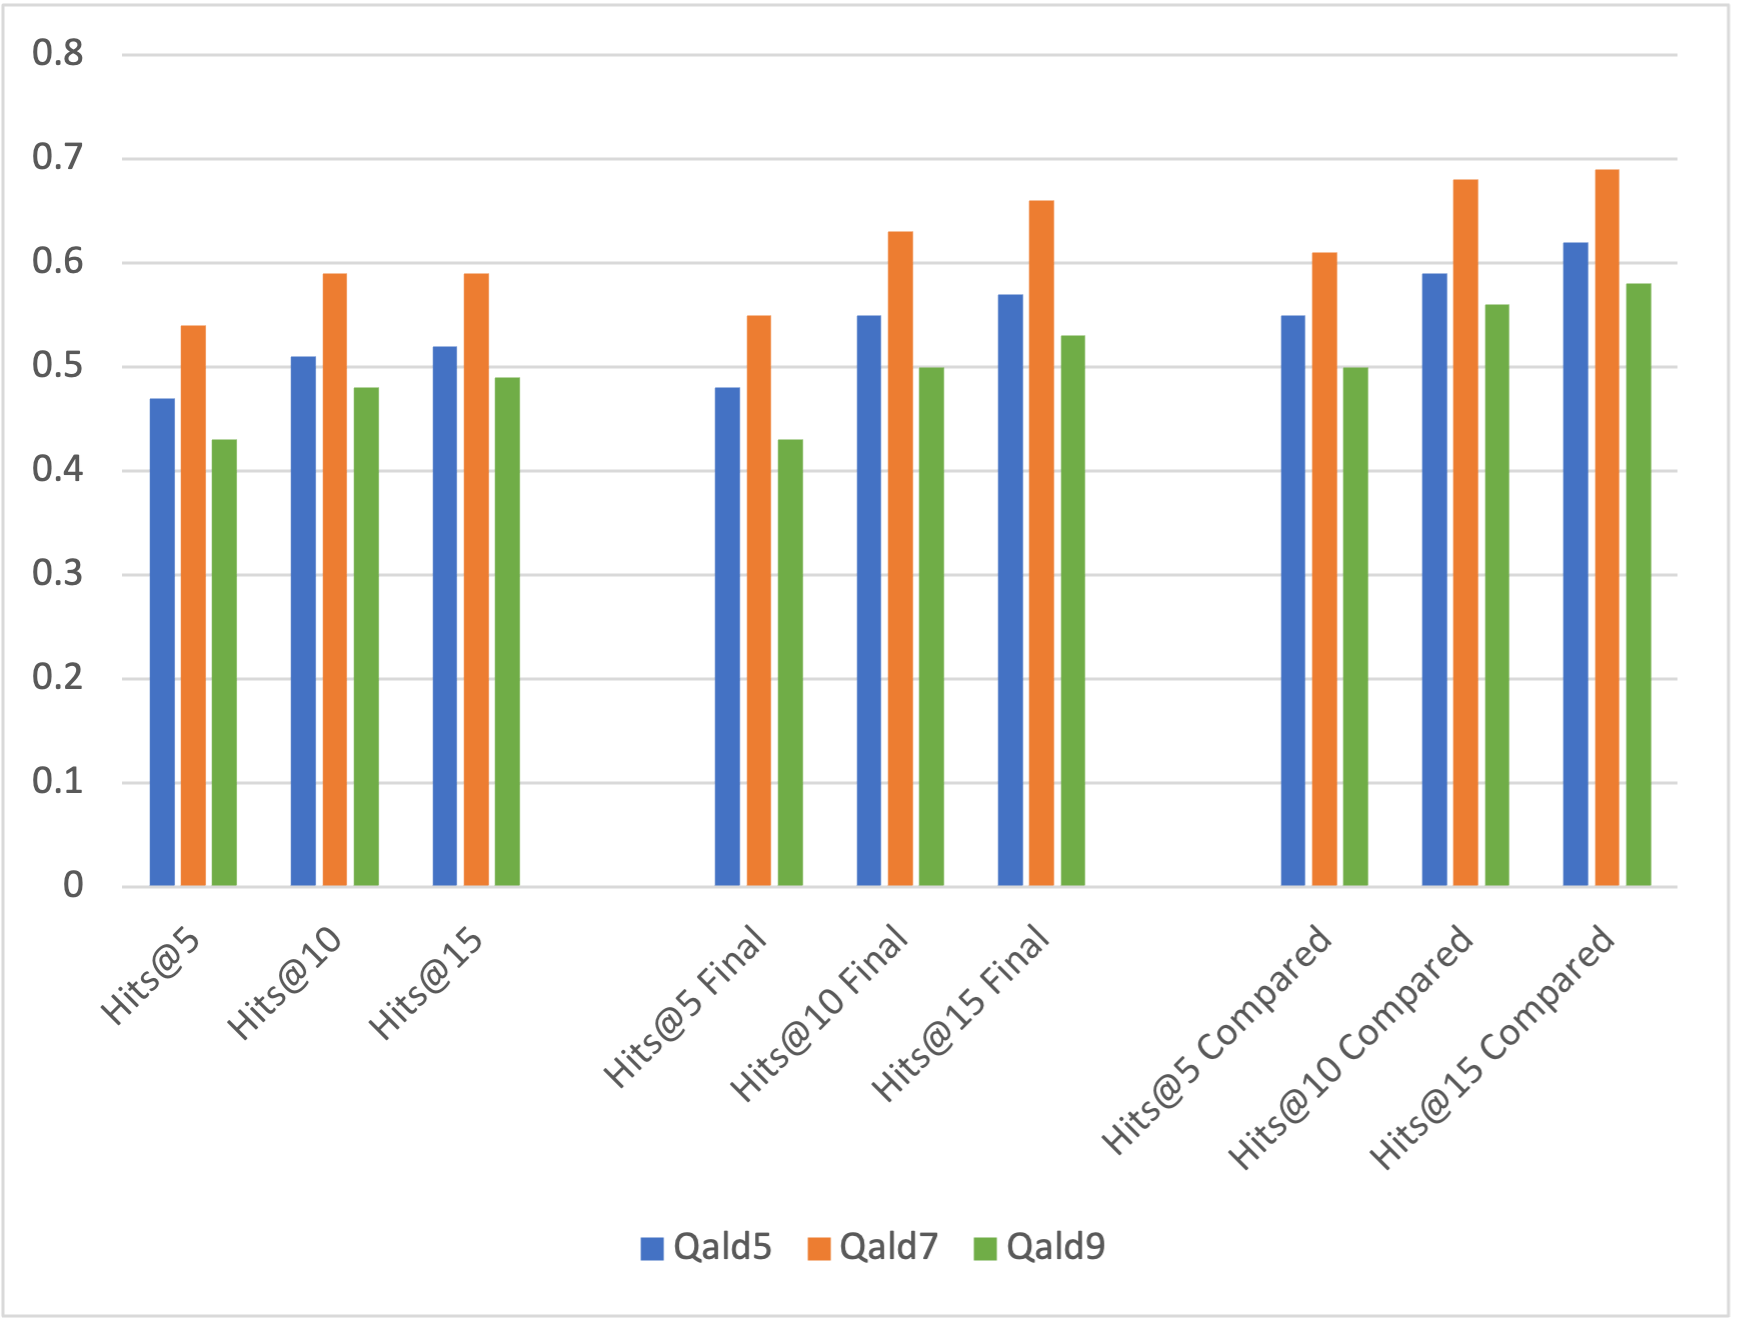
\includegraphics[width=12cm, height=7cm]{chapters/figures/qaldresults.png}
%     \caption{Approach}
%     \label{fig:results}
% \end{figure}

\cite{chen_shen_huang_wang_2021}\cite{OpenTapioca}\cite{Weichselbraun}\cite{tagme}